\documentclass[11pt]{beamer}
\usetheme{Boadilla}
\usepackage[utf8]{inputenc}
\usepackage{amsmath}
\usepackage{amsfonts}
\usepackage{amssymb}
\graphicspath{{../fig/}{../Feynman/}}
%\author{}
\title{Updates on the new implementation of LPM effect}
%\setbeamercovered{transparent} 
%\setbeamertemplate{navigation symbols}{} 
%\logo{} 
%\institute{} 
%\date{} 
%\subject{} 
\begin{document}

\begin{frame}
\titlepage
\end{frame}

%\begin{frame}
%\tableofcontents
%\end{frame}

\begin{frame}{Build the model}
\begin{overprint}
\onslide<1>
\vspace{1cm}
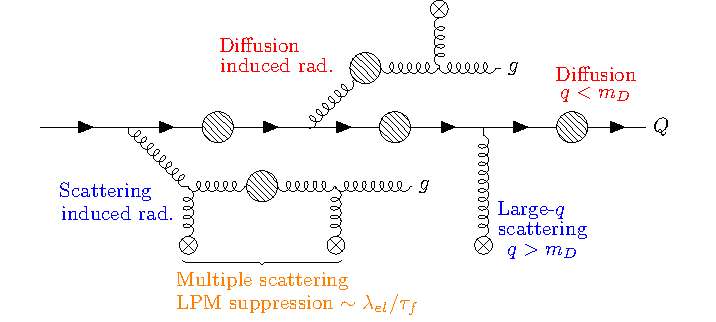
\includegraphics[width=\textwidth]{all-processes.pdf}
\onslide<2>
\vspace{1cm}
\begin{itemize}
\item $Q+q \rightarrow Q+q$ and $Q+g \rightarrow Q+g$.
\item Restrict to large momenta transfer $|t| > m_D^2$.
\end{itemize}
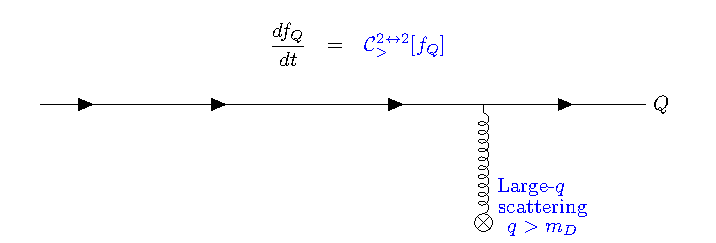
\includegraphics[width=.9\textwidth]{22.pdf}
\onslide<3>
\vspace{1cm}
\begin{itemize}
\item Diffusion coefficient $\kappa \propto \alpha_s^2 T^3 \ln(1+Q_{\max}^2/m_D^2)$.
\item Small momenta transfer $|t| < m_D^2$, $Q_{\max}^2=m_D^2$.
\item Solved by Langevin Equation. Drag defined by the Einstein relation.
\end{itemize}
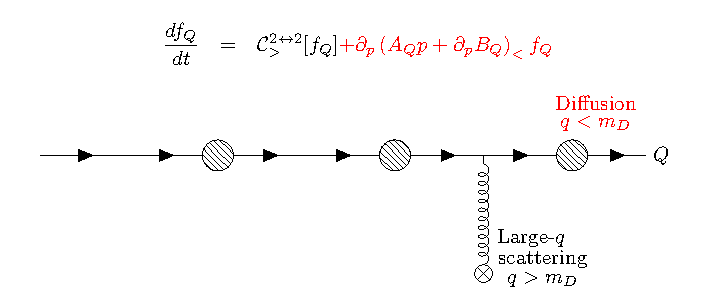
\includegraphics[width=.9\textwidth]{22-11.pdf}
\onslide<4>
\vspace{1cm}
\begin{itemize}
\item Incoherent processes: $Q+q\rightarrow Q+q+g$ and $Q+g\rightarrow Q+g+g$.
\item Gunion-Bertsch matrix-element, $|M_{23}|^2 = |M_{22}|^2 |M_{12}|^2$
\item Restrict to large momenta transfer $|t| > m_D^2$ in $|M_{22}|^2$.
\end{itemize}
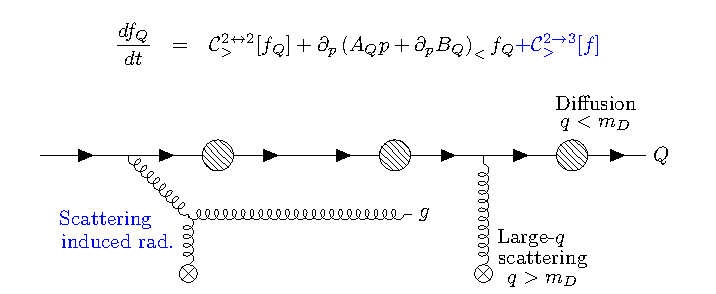
\includegraphics[width=.9\textwidth]{22-11-23.pdf}
\onslide<5>
\vspace{.5cm}
\begin{itemize}
\item Incoherent processes: diffusion induced $Q \rightarrow Q+g$.
\vspace{-.25cm}
\begin{equation}
\nonumber
dR_{12} = \hat{q}_{g,<} \frac{\alpha_s}{2\pi}P(x)dx \frac{dk_\perp^2}{k_\perp^4}
\end{equation} 
\vspace{-.5cm}
\item Restrict to large momenta transfer $|t| > m_D^2$ in $|M_{22}|^2$.
\end{itemize}
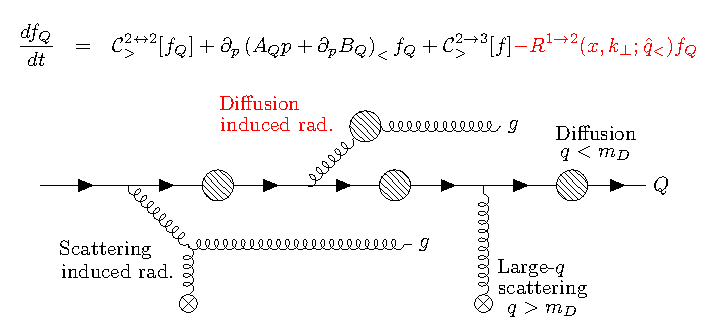
\includegraphics[width=.9\textwidth]{22-11-23-12.pdf}
\onslide<6>
Implement LPM effect by rejecting incoherent gluon radiation.\\
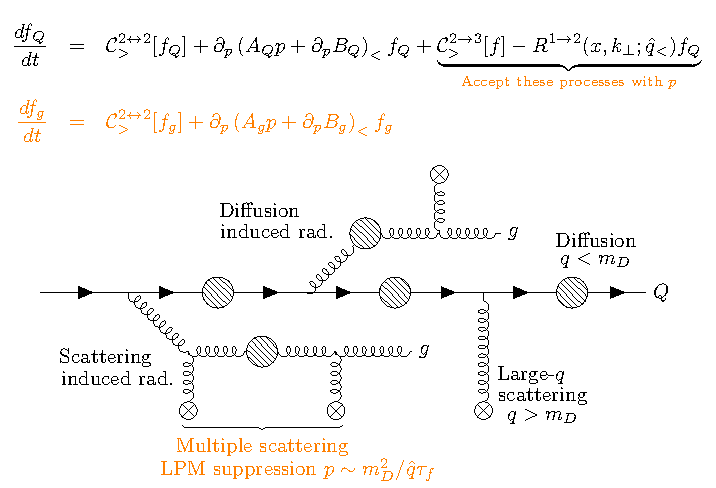
\includegraphics[width=.9\textwidth]{22-11-23-12-lpm.pdf}
\end{overprint}
\end{frame}

\begin{frame}{Running coupling and dead-cone effect}
Running coupling constant
\begin{itemize}
\item Process generated with $\alpha_s(k_{\perp,i}^2)$. 
\item But the final transverse momentum $k_{\perp,f}^2 > k_{\perp,i}^2$.
\item Modify the acceptance $p' = p\frac{\alpha_s(k_{\perp,f}^2)}{ \alpha_s(k_{\perp,i}^2)}$.
\end{itemize}
Mass (Dead-cone) effect
\begin{itemize}
\item Radiation off heavy quark is suppressed when $\theta < \theta_D = M/E$
\item Further modify the acceptance $p'' = p' \left(\frac{\theta^2}{\theta^2 + \theta_D^2} \right)^n$.
\end{itemize}
\end{frame} 


\begin{frame}{Performance: infinite medium limit}
\begin{itemize}
\item Ratio of spectrum $dI/d\omega$ to theory.
\item $\omega < 2\pi T$, go back to incoherent limit.
\item $\omega > 2\pi T$, agree with AMY-NLL spectrum within $\pm 15\%$
\end{itemize}
\begin{overprint}
\onslide<1>
\begin{center}
$\alpha_s = 0.1$\\
\includegraphics[width=.6\textwidth]{spectrum_E_alphas0d1.pdf}
\end{center}
\onslide<2>
\begin{center}
$\alpha_s = 0.3$\\
\includegraphics[width=.6\textwidth]{spectrum_E_alphas0d3.pdf}
\end{center}
\end{overprint}
\end{frame}

\begin{frame}{Performance: finite medium}
\begin{itemize}
\item Spectrum $dI/d\omega$ dependents on path-length $L$.
\item Simulation well reproduce the full theory calculation.
\end{itemize}
\begin{center}
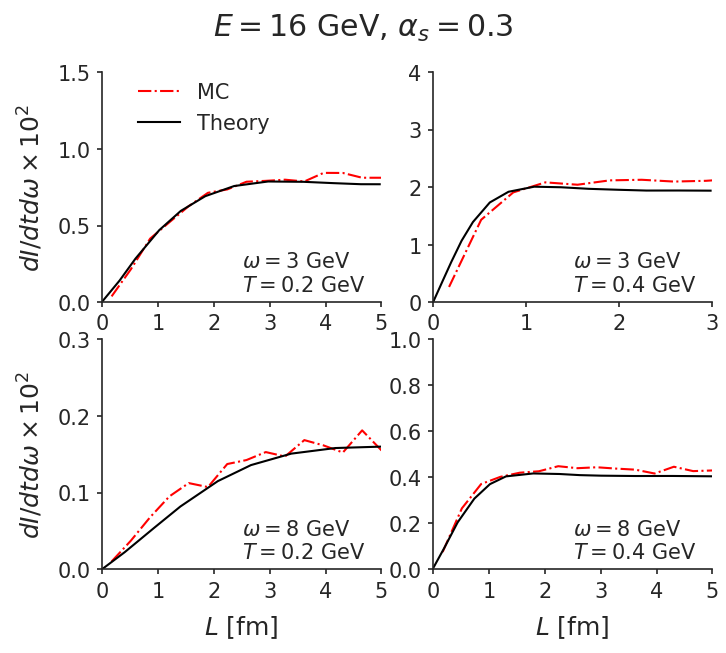
\includegraphics[width=.6\textwidth]{spectrum_L.pdf}
\end{center}
\end{frame}




\end{document}